\subsection{Einleitung}
Im Rahmen der PeP et al. Sommerakademie 2013 wurde unter anderem das Projekt \enquote{Wasserrakete} durchgeführt. Ziel war es, eine Rakete samt Abschussbasis zu konstruieren, angetrieben durch Druckluft mit Wasser als Stützmittel. 
\subsection{Bau}
Für den Bau von Rakete und Abschussbasis werden folgende Materialien benötigt:
\begin{itemize}
\item Cola-Flasche
\item Gardena Hahnanschluss+Schlauchkupplung
\item 2 Plastikdeckel von Haribo-Schachteln für die Finnen
\item Wollgarn
\item Nylonfaden
\item \emph{viel} Gaffertape
\item Zwei-Komponenten-Kleber (z.B. UHU Endfest 300)
\item Tennisball
\item Tischtennisball
\item 2te Plastikflasche
\item ca. 20\,cm Dachlatte
\item Fahradreifenventil mit Adapter auf Autoreifenventil
\item 4 L-Winkel aus Metall
\item Fotostativ mit herausnehmbarer Mittelsäule oder 3-4 60\,cm Dachlatten
\item M5-Schrauben mit passenden Gegenmuttern
\item Schraubösen
\item Fahrradpumpe mit Autoventilöffnung
\end{itemize}
\subsection{Rakete}

Die Flasche dient als Tank und Korpus der Rakete, da das Anschlussstück des Hahnanschlusses nicht auf das Gewinde der Flasche passt, muss dieses abgesägt werden. Hierbei sollte möglichst viel Material an der Flasche verbleiben.
Das Anschlussstück wird nun mit dem Zwei-Komponentenkleber an die Flasche geklebt, die Trocknungszeit bei dem hier verwendeten Kleber beträgt ca. 24 Stunden. 
Aus den Deckeln der Süßigkeitendosen werden vier Finnen ausgeschnitten und symmetrisch an die Unterseite der Rakete geklebt. Hierfür wird zunächst der Zwei-Koponentenkleber verwendet und nach Austrocknung wird noch einmal mit Gaffertape fixiert.
Für die Spitze der Rakete wurden mehrere Materialien getestet:
\begin{enumerate}
\item Tennisball, passt genau in die Bodenvertiefung der Flasche $\Rightarrow$ unnötig hohes Gewicht
\item keine Spitze $\Rightarrow$ Schäden an der Raketenspitze, undicht
\item Rundung einer PET-Flasche mit halben Tischtennisball als Spitze (*)
\end{enumerate}


\subsection{Abschussvorrichtung}

Für den Abschussmechanismus muss zunächst das Fahrradreifenventil in den unteren Teil (mit dem beweglichen, orangenem Mantel) des Hahnanschlusses geklebt werden. Dazu wird die Gewindemutter des Fahrradventils bündig mit der unteren Öffnung der Schlauchkupplungverklebt. Wenn der Zwei-Komponentenkleber getrocknet ist, wird von der Gegenseite ein Autoadapter auf das Fahrradventil geschraubt. Dadurch wird das Fahrradventil zusätzlich fixiert.
 Die vier L Winkel werden mit Schrauben und passenden Gegenmuttern so zusammengeschraubt, dass das Anschlussstück in einem Ring eingeschlossen wird. Dafür muss ein zusätzliches Loch in das Metall gebohrt werden. Die L-Winkel werden zwischen der grauen Plastikmutter und dem Gewindekranz der Schlauchkupplung eingeklemmt.


Ein Bild des Abschussmechanismusses ist in Abbildung \ref{fig:ausloeser} zu sehen.




\subsection{Erste Tests}
Bei den aller ersten Tests bestand die Rakete lediglich aus der Plastikflasche (mit Hahnanschluss). Mit einem Druck von 2\,bar und einem Wasservolumen von ca. 300\,ml startete die Rakete direkt beim ersten Versuch erfolgreich. Nach einigen Starts mit gleichem Druck gab die Hahnanschluss-Klebestelle schon bei einer geringen Druckerhöhung nach.\\
Es folgte eine Überarbeitung der Rakete, bei der der Hahnanschluss, die Finnen und der Tennisball an die Flasche geklebt wurden. Zusätzlich wurde eine Schnur an der Rakete befestigt, mit der die Flughöhe näherungsweise bestimmt werden konnte.\\ %Bild von überarbeitete Rakete 
Nachdem der Kleber ausgetrocknet war, starteten die nächsten Versuche. Nach dem ersten erfolgreichen Start fiel der Tennisball bei der Landung jedoch ab. Deshalb fanden die folgenden Tests ohne Tennisball statt. Dies führte dazu, dass ein paar Starts später die Spitze der Rakete (der Boden der Flasche) auf der naheliegenden Starße aufschlug und so ein Riss entstand. Da aus diesem Luft entwich, musste die Rakete erst wieder überarbeitet werden. Bei den bis dahin durchgeführten Tests wurden bereits Höhen von ca. 10\,m erreicht.\\
Die Rakete wurde weiter modifiziert. Neben dem Flicken des Risses wurde die austauschbare Schutzhaube (*) zur Verbesserung der Aerodynamik und zum Abfangen des Sturzes angeklebt.\\ 
Um auszuprobieren bis zu welchem Druck man gehen kann, wurde eine zweite Rakete, bestehend aus einer 1,5\,l-Einweg-PET-Flasche und einem Hahnanschluss, gefertigt.\\
Im dritten Durchgang bewiesen sich die Raketen als soweit zuverlässig, dass mit den Messreihen begonnen werden konnte.


\subsection{Messreihen}
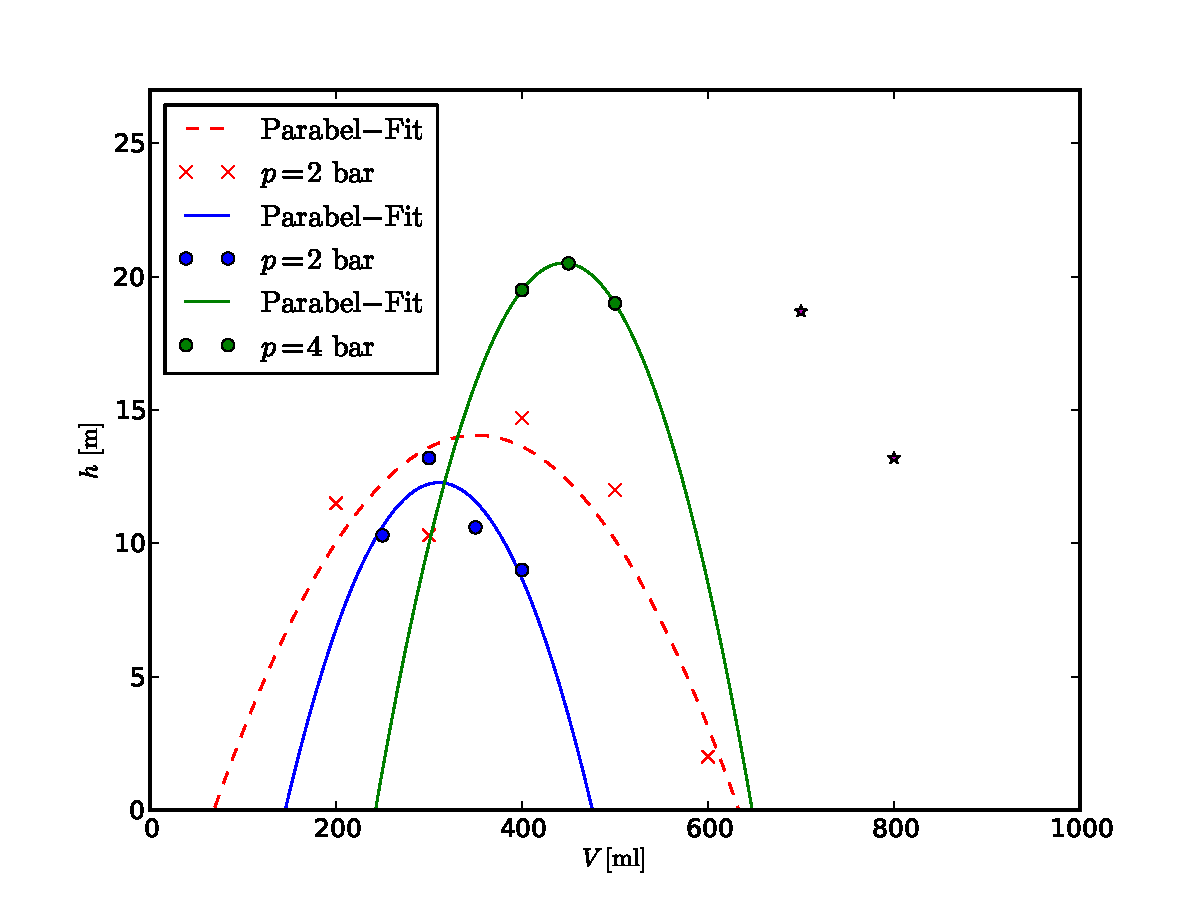
\includegraphics[width=\textwidth]{figs/rakete/raketenplot.pdf}
Ende der Testreihe:
\begin{enumerate}
\item bei einem Druck von 7\,bar öffnete sich der geflickte Riss in der Raketenspitze der Hauptrakete wieder
\item die zusätzliche Rakete explodierte unter 8\,bar
\end{enumerate}


\subsection{Zusammenfassung}
Die Raketen waren flugtauglich. Es konnten sowohl Messreihen in Abhängigkeit des Wasservolumens in der Rakete, als auch in Abhängigkeit des Druckes durchgeführt werden. 
%auf Messreihen eingehen

\subsection{Verbesserungen}
\begin{enumerate}
\item längeren Schlauch für die Luftpumpe
\item Schutzausrüstig (wie Brille und Ohrenschützer)
\item größere Klebeflächen
\item Stabilisierung der Gartenschlauchkupplungshalterung
\item Fallschirm an Raketenspitze anbringen?
\end{enumerate}

\begin{figure}[!h]
\centering
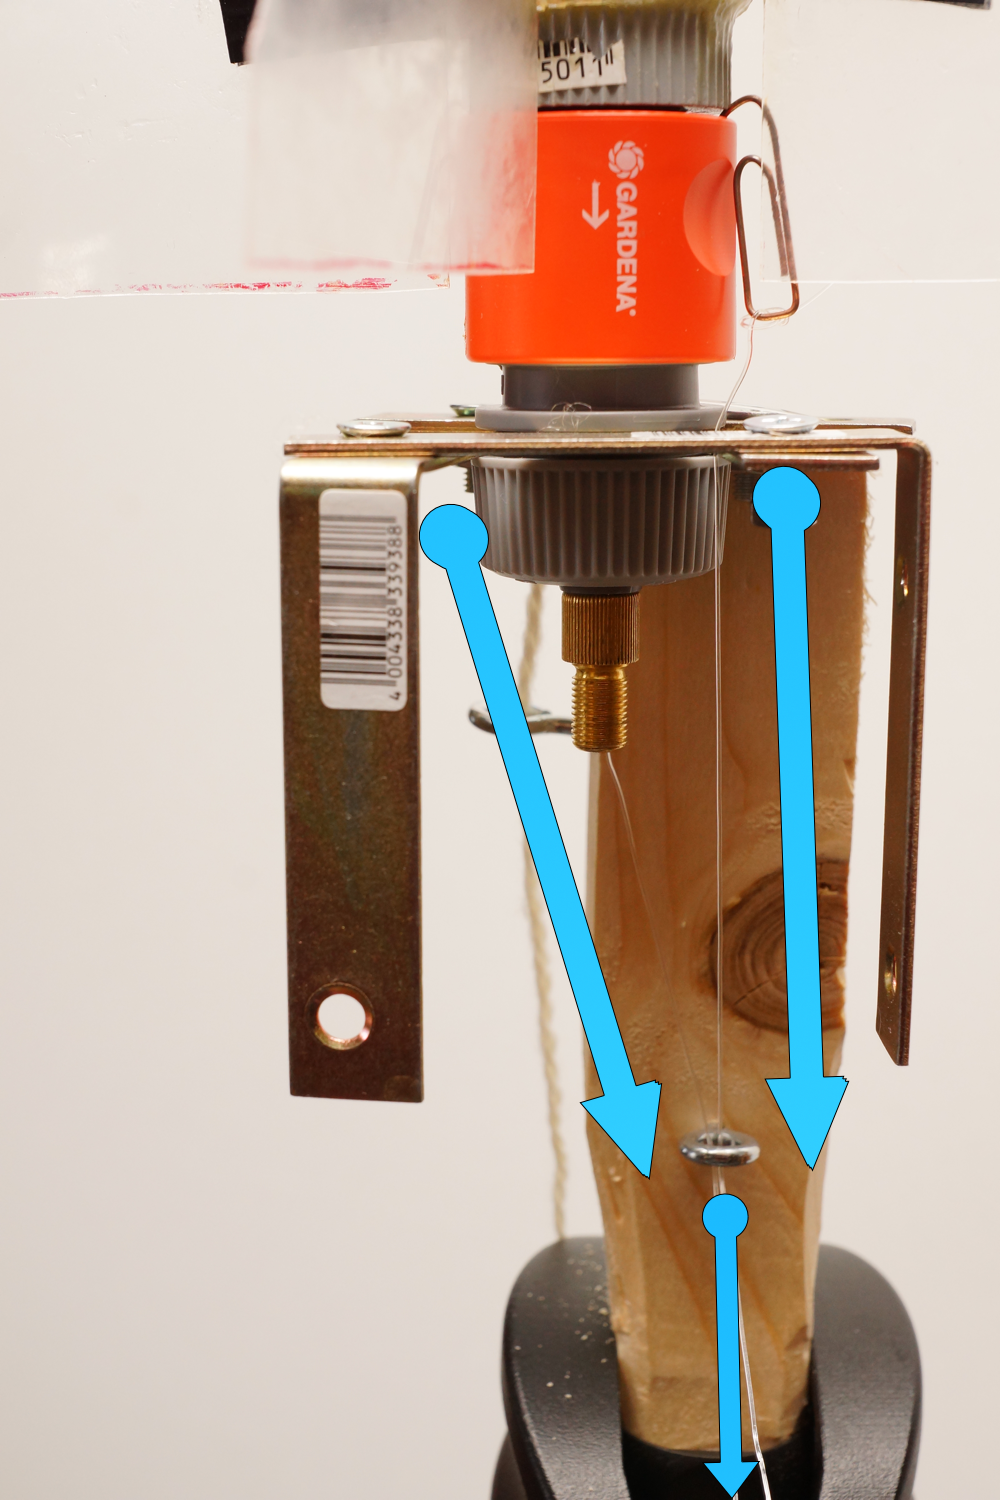
\includegraphics[width=10cm]{figs/rakete/ausloesemechanismus.png}
\caption{Auslösemechanismus mit Rakete}\label{fig:ausloeser}
\end{figure}